\documentclass[12pt,aspectratio=169]{beamer}
\usetheme{metropolis}
\setbeamersize{text margin left=.5cm,text margin right=.5cm}
\usepackage[lf]{carlito}
\usepackage{siunitx}
\usepackage{tikz}
\usepackage{mathpazo}
\usepackage{bm}
\usepackage{mathtools}
\usepackage[ISO]{diffcoeff}
\diffdef{}{ op-symbol=\mathsf{d} }
\usepackage{xcolor,colortbl}

\setmonofont{Ubuntu Mono}
\setlength{\parskip}{0pt}
\renewcommand{\baselinestretch}{1}

\sisetup{
  inter-unit-product=\cdot,
  per-mode=symbol
}

\tikzset{
  >=latex
}

%\newcommand{\iii}{\hat{\bm\imath}}
%\newcommand{\jjj}{\hat{\bm\jmath}}
%\newcommand{\kkk}{\hat{\bm k}}

\usepackage[siunitx]{circuitikz} % to draw circuits!

\title{Class 16: Faraday's Law \& Magnetic Induction}
\subtitle{Advanced Placement Physics C}
\author[TML]{Dr.\ Timothy Leung}
\institute{Olympiads School}
\date{Updated: Summer 2022}

\newcommand{\pic}[2]{
  \includegraphics[width=#1\textwidth]{#2}
}
\newcommand{\eq}[2]{
  \vspace{#1}{\Large
    \begin{displaymath}
      #2
    \end{displaymath}
  }
}
%\newcommand{\iii}{\ensuremath\hat{\bm{\imath}}}
%\newcommand{\jjj}{\ensuremath\hat{\bm{\jmath}}}
%\newcommand{\kkk}{\ensuremath\hat{\bm{k}}}
\newcommand{\iii}{\ensuremath\hat\imath}
\newcommand{\jjj}{\ensuremath\hat\jmath}
\newcommand{\kkk}{\ensuremath\hat k}



\begin{document}

\begin{frame}
  \maketitle
\end{frame}


\section{Faraday's Law}

\begin{frame}{Magnetic Flux}
  \textbf{Question:} If a current-carrying wire can generate a magnetic field,
  can a magnetic field affect the current in a wire?

  \vspace{.3in}\textbf{Answer:} Yes, sort of\ldots

  \vspace{.3in}To understand how to \emph{induce} a current by a magnetic field,
  we need to look at fluxes again.
\end{frame}


\begin{frame}{Magnetic Flux}
  \begin{columns}
    \column{.4\textwidth}
    \pic1{flux2}
  
    \column{.6\textwidth}
    Magnetic flux is defined as:
    
    \eq{-.15in}{
      \boxed{\Phi_m=\int\vec B\cdot\dl\vec A}
    }
    
    where $\vec B$ is the magnetic field, and $\dl\vec A$ is the infinitesimal
    area pointing \textbf{outwards}. Note that magnetic flux can also be
    expressed as:

    \eq{-.2in}{
      \boxed{\Phi_m=\int\vec B\cdot\hat n\dl A}
    }

    where $\hat n$ is the outward normal direction
  \end{columns}
\end{frame}



\begin{frame}{Magnetic Flux Over a Closed Surface}
  The SI unit for magnetic flux is a ``weber'' (\si\weber), in honor of German
  physicist Wilhelm Weber, who invented the electromagnetic telegraph with Carl
  Gauss. The unit is defined as:

  \eq{-.23in}{
    \SI1\weber=\SI1{\tesla\metre\squared}
  }
  
  \vspace{-.15in}The magnetic flux over a closed surface is always zero
  (\textbf{Gauss's law for magnetism}):

  \eq{-.15in}{
    \boxed{\oint\vec B\cdot\dl\vec A=0}
  }

  Since magnetic field lines only exist as a loop, that means there should be
  equal amount of ``flux'' flowing out of a closed surface as entering the
  surface.
\end{frame}


\begin{frame}{Changing Magnetic Flux}
  Changes to magnetic flux can be due to a number of reasons:
  \begin{enumerate}
  \item\textbf{Changing magnetic field} $\vec B$: the magnetic field is
    created by a time-dependent source (e.g.\ alternating current)
  \item\textbf{Changing area} $A$: the surface area from which the flux is
    calculated is changing
  \item\textbf{Changing orientation of magnetic field} $\vec B\cdot\dl\vec A$:
    the surface area is moving relative to the magnetic field
  \end{enumerate}
\end{frame}



\begin{frame}{Faraday's Law}
  \textbf{Faraday's law} states that the rate of change of magnetic flux
  produces an electric field $\vec E$ in a circuit, and therefore an
  electromotive force $\mathcal E$ (voltage):

  \eq{-.2in}{
    \boxed{
      \mathcal E=\oint\vec E\cdot\dl\vec\ell={\color{red}{-}}
      \diff{\Phi_m}t
    }
  }
  
  The negative sign {\textcolor{red}{highlighted in red}} is the result of
  \textbf{Lenz's law}, which is related to the conservation energy
\end{frame}





\begin{frame}{When Magnetic Flux is Changing}
  \begin{itemize}
  \item When the magnetic flux $\Phi_m$ is changing, an electromotive force
    (\emph{emf}, $\mathcal E$) is created in the wire.
  \item Unlike in a circuit, where the \emph{emf} is concentrated at the
    terminals of the battery, the induced \emph{emf} is spread across the
    entire wire.
  \end{itemize}
  \begin{columns}
    \column{.3\textwidth}
    \begin{center}
      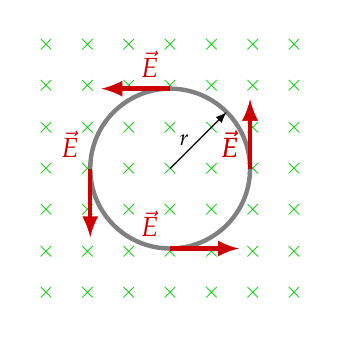
\begin{tikzpicture}[scale=.35]
        \foreach \xx in {-4.5,-3,...,4.5}{
          \foreach \yy in {-4.5,-3,...,4.5}{
            \node at (\xx,\yy)
                  {\footnotesize\textcolor{green!80!black}{$\times$}};
          }
        }
        \draw[gray,ultra thick](0,0) circle(2.9);
        \draw[->,rotate=45](0,0)--(2.9,0) node[midway,left]{\footnotesize $r$};
        \foreach \x in {0,90,...,360} {
          \begin{scope}[rotate=\x]
            \draw[ultra thick,red!80!black,->](2.9,0)--(2.9,2.5)
            node[pos=0,above left]{$\vec E$};
          \end{scope}
        }
      \end{tikzpicture}
    \end{center}
    
    \column{.7\textwidth}
    \begin{itemize}
    \item Since \emph{emf} is work per unit charge, that means that there is an
      electric field inside the wire to move the charges.
    \item In this example:
      \begin{itemize}
      \item Magnetic field $\vec B$ into the page
      \item The direction of the electric field $\vec E$ corresponds to an
        \emph{increase} in magnetic flux
      \end{itemize}
    \end{itemize}
  \end{columns}
\end{frame}


\begin{frame}{AC Generators}
  A simple AC (alternating current) generator makes use of the fact that a 
  coil rotating against a fixed magnetic field has a changing flux.
  \begin{center}
    \pic{.45}{generator}
  \end{center}
  Let's say the permanent magnets produce a uniform magnetic field $B$, and the
  coil between them has $N$ turns, and an area $A$. Now let's say that the coil
  is rotating with an angular frequency $\omega$.
\end{frame}



\begin{frame}{AC Generators}
  \begin{columns}
    \column{.35\textwidth}
    \pic1{generator}

    \column{.65\textwidth}
    When the coil is turning, the angle between the coil and the magnetic field
    is:
    
    \eq{-.2in}{
      \theta=\omega t+\delta
    } 

    \vspace{-.1in}where $\delta$ is the initial angle. The magnetic flux
    through the coil is given by:
    
    \vspace{-.4in}{\Large
      \begin{align*}
        \Phi_m&=NBA\cos\theta\\
        &=NBA\cos(\omega t+\delta)
      \end{align*}
    }
    
    \vspace{-.3in}as the coil turns.
  \end{columns}
\end{frame}



\begin{frame}{AC Generators}
  \begin{columns}
    \column{.33\textwidth}
    \pic{1.05}{generator}

    \column{.67\textwidth}  
    The electromotive force \emph{emf} produced is therefore the rate of change
    of the magnetic flux:

    \vspace{-.3in}{\Large
      \begin{align*}
        \mathcal E &=-\diff{\Phi_m}t\\
        &=\underbracket{NBA\omega}_{\mathcal E_\text{max}}\sin(\omega t+\delta)
      \end{align*}
    }
  \end{columns}
\end{frame}



%\begin{frame}{AC Generators}
%  \begin{columns}
%    \column{.35\textwidth}
%    \pic1{generator}
%
%    \column{.65\textwidth}
%    We commonly write it this way instead:
%    
%    \eq{-.25in}{\mathcal{E}=\mathcal{E}_{\textrm{max}}\sin(\omega t+\delta)}
%    
%    \vspace{-.2in}where
%
%    \eq{-.25in}{
%      \mathcal{E}_{\textrm{max}}=NBA\omega
%    }
%  \end{columns}
%\end{frame}



\begin{frame}{Motional EMF}
  {What happens when I slide the rod to the right?}
  \begin{columns}
    \column{.45\textwidth}
    \pic1{motional-emf-1}

    \column{.55\textwidth}
    When sliding the rod to the right with speed $v$, the magnetic flux through
    the loop (and its rate of change) is:

    \vspace{-.4in}{\Large
      \begin{align*}
        \Phi_m &=BA=B\ell x\\
        \diff{\Phi_m}r &= B\ell\diff xt=\boxed{B\ell v=\mathcal E}
      \end{align*}
    }
    
    We can use the Lorentz force law on the charges on the rod to find the
    direction of the current $I$.
  \end{columns}
\end{frame}



\begin{frame}{Motional EMF}{What happens when I slide the rod to the right?}
  \begin{columns}
    \column{.22\textwidth}
    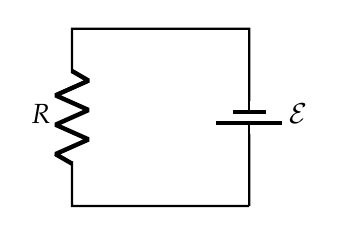
\begin{tikzpicture}[scale=1.5]
      \draw[thick](1.5,0) to[battery1,l_=$\mathcal E$] (1.5,1.5)--(0,1.5)
      to[R,l_=$R$] (0,0)--(1.5,0);
    \end{tikzpicture}
    
    \column{.78\textwidth}
    \begin{itemize}
    \item An equivalent circuit is shown on the left
    \item The amount of current can be found using Ohm's law: $V=IR$
    \item Note that the ``motional emf'' produced is spread over the entire
      circuit
      \begin{itemize}
      \item In constrast, in a voltaic cell (or battery), the \emph{emf} is
        concentrated between the two terminals.
      \end{itemize}
    \end{itemize}
  \end{columns}
\end{frame}



\section{Lenz's Law}

\begin{frame}{Lenz's Law}
  Something very interesting happens when the current starts running on the
  wire.
  \begin{center}
    \pic{.35}{motional-emf-2}
  \end{center}
  It produces an ``induced magnetic field'' out of the page, in the opposite
  direction as the field that generated the current in the first place.
\end{frame}



\begin{frame}{Lenz's Law}
  \begin{center}
    \fbox{
      \begin{minipage}{.7\textwidth}
        \textbf{LENZ'S LAW}\\
        The induced \emph{emf} and induced current are in such are
        direction as to oppose the change that produces them
      \end{minipage}
    }
  \end{center}

  \vspace{.2in}So basically, the conservation of energy
\end{frame}



\section{Inductance}

\begin{frame}{Back \emph{emf}}
  Consider a very simple circuit consisting of a voltage source and a coil
  \begin{center}
    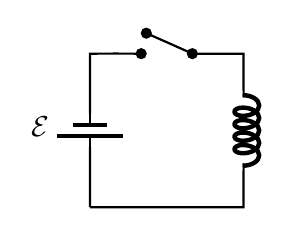
\begin{tikzpicture}[american voltages,scale=1.3]
      \draw[thick](0,0) to[battery1,l=$\mathcal E$] (0,1.5)
      to[short,-*](.5,1.5);
      \draw[thick](.55,1.7) to[short,*-*](1,1.5)--(1.5,1.5)
      to[L] (1.5,0)--(0,0);
    \end{tikzpicture}
  \end{center}
  \begin{itemize}
  \item When the switch is closed and current begins to flow, the coil
    begins to generate a magnetic flux inside
  \item As the current changes (initially increasing with time), it
    self-induces a ``back \emph{emf}'' that opposes the change in current
  \item A current can't jump from zero to some value (or from some value to
    zero) instantaneously
  \end{itemize}
\end{frame}



\begin{frame}{Back \emph{emf}}
  \begin{center}
    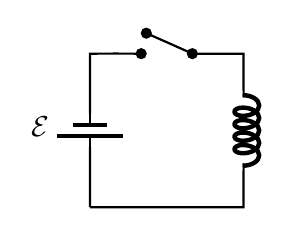
\begin{tikzpicture}[american voltages,scale=1.3]
      \draw[thick](0,0) to[battery1,l=$\mathcal E$] (0,1.5)
      to[short,-*](.5,1.5);
      \draw[thick](.55,1.7) to[short,*-*](1,1.5)--(1.5,1.5)
      to[L] (1.5,0)--(0,0);
    \end{tikzpicture}
  \end{center}
  \begin{itemize}
  \item Breaking the circuit causes the magnetic flux to change very rapidly
  \item The rapid change of $\Phi_m$ creates a large induced back \emph{emf}
    that is proportional to the time rate of change of magnetic flux
    $\Phi_m'(t)$
  \item The back \emph{emf} creates a large voltage drop across the switch
  \item Large voltage across two metal contact produces a very strong electric
    field--strong enough to tear electrons away from air molecules
    (``dielectric breakdown'')
  \item Air conducts electricity in the form of a ``spark''
  \end{itemize}
\end{frame}



\begin{frame}{Self Inductance}
  A solenoid carrying a current generates a magnetic field $B$; its magnitude at
  the core is proportional to the current $I$:

  \eq{-.2in}{
    B=\left[\frac{\mu_0N}\ell\right]I
  }

  Since $\vec B\propto I$, the magnetic flux through the core of the solenoid
  (really $\Phi_m=NBA$, where $A$ is the cross-sectional area of the solenoid
  and $N$ is the number of coils) is therefore also proportional to $I$, i.e.

  \eq{-.2in}{
    \boxed{\Phi_m=LI}
  }

  where $L$ is the called the \textbf{self inductance} of the coil.
\end{frame}



\begin{frame}{Self Inductance}
  For a solenoid, we can see that the self inductance is given by:

  \eq{-.2in}{
    \boxed{L=\frac{\Phi_m}I=\mu_0 n^2A\ell}
  }

  \begin{center}
    \begin{tabular}{l|c|c}
      \rowcolor{pink}
      \textbf{Quantity} & \textbf{Symbol} & \textbf{SI Unit} \\ \hline
      Self inductance                    & $L$     & \si\henry\\
      Vacuum permeability                & $\mu_0$ & \si{T.m/A} \\
      Number of coils per unit length    & $n$     & \si\ampere \\
      Cross-section area of the solenoid & $A$     & \si{\metre\squared} \\
      Length of the solenoid             & $\ell$  & \si\metre
    \end{tabular}
  \end{center}
  Note that $A\ell$ is the \emph{enclosed volume} of the solenoid.
\end{frame}



\begin{frame}{Self Inductance and Induced EMF}
  If the current changes, the magnetic flux changes as well, therefore inducing
  an electromotive force in the circuit According Faraday's law:

  \eq{-.1in}{
    \boxed{\mathcal E=-\diff {\Phi_m}t=-L\diff It}
  }

  The self-induced \emph{emf} is proportional to the rate of change of current
\end{frame}



\begin{frame}{Magnetic Energy}
  At any instant, the magnitude of the induced emf is

  \eq{-.2in}{
    \mathcal{E}=L\diff It
  }
  so the power absorbed by the inductor is

  \eq{-.2in}{
    P(t)=\mathcal EI=LI\diff It
  }

  Integrating in time gives the magnetic (potential) energy that is stored in
  the magnetic field:

  \eq{-.2in}{
    U_m
    =\int_0^t P(\tau)\dl\tau
    =L \int I\diff I\tau \dl\tau
    =L \int_0^I I\dl I=\frac12LI^2
  }
\end{frame}



\begin{frame}{Magnetic Energy}
  Just as a capacitor stores energy in its electric field, an inductor coil
  carrying a current $I$ stores energy in its magnetic field, given by:

  \eq{-.2in}{
    \boxed{U_m=\frac12LI^2}
  }

  We can also define a \textbf{magnetic energy density}:

  \eq{-.2in}{
    \boxed{\eta_m=\frac{B^2}{2\mu_0}}
  }
\end{frame}


%\section{LC Circuit}
%\begin{frame}
%  \frametitle{LC Circuit}
%  The final type of circuit that we will study in AP Physics is the LC
%  circuit. In its simplest form, the circuit has an inductor and capacitor
%  connected in series:
%  \begin{center}
%    \begin{tikzpicture}[american voltages,scale=1.2]
%      \draw[thick](0,0) to[L=$L$] (0,2)--(2,2) to[C=$C$] (2,0)--(0,0);
%    \end{tikzpicture}
%  \end{center}
%  We apply the Kirchkoff's voltage law:
%  
%  \eq{-.2in}{
%    -V_L-V_C=0
%    \quad\rightarrow\quad
%    L\frac{dI}{dt}+\frac{Q}{C}=0
%  }
%\end{frame}
%
%\begin{frame}
%  \frametitle{LC Circuits}
%  Since both terms are continuously differentiable, we can differentiate both
%  sides of the equation, which gives:
%
%  \eq{-.2in}{
%    L\frac{d^2I}{dt^2}+\frac1{C}\underbrace{\frac{dQ}{dt}}_I=0
%  }
%
%  In fact, the above equation is one that we have studied many topics ago:
%
%  \eq{-.2in}{
%    \frac{d^2I}{dt^2}+\frac1{LC}I=0
%  }
%
%  This is a second-order ordinary differential equation, and the solution is
%  the simple harmonic motion.
%\end{frame}
%
%
%\begin{frame}
%  \frametitle{LC Circuit}
%  The current inside of an LC circuit is given by:
%
%  \eq{-.2in}{
%    I(t)=I_0\sin(\omega t + \varphi)\quad\text{where}\quad
%    \omega=\frac1{\sqrt{LC}}
%  }
%\end{frame}
%
\end{document}
